\documentclass{acmlarge}

\usepackage{multibib}
\newcites{adx}{Appendix Citations}


%\usepackage{showframe}
% Support for CCSXML file
\RequirePackage{comment}
\excludecomment{CCSXML}

% New concepts scheme
%
% The first argument is the significance, the
% second is the concept(s)
%
% https://dl.acm.org/ccs.cfm?
\makeatletter
\let\@concepts\@empty

\def\category#1#2#3{\@ifnextchar
  [{\@category{#1}{#2}{#3}}{\@xcategory{#1}{#2}{#3}}}
\def\@category#1#2#3[#4]{\edef\@tempa{\ifx \@concepts\@empty 
    \else ; \fi}{\def\protect{\noexpand\protect
      \noexpand}\def\and{\noexpand\and}\xdef\@concepts{\@categories\@tempa #1
      [{\bf #2}]: 
      #3\kern\z@---\hskip\z@{\it #4}}}}
\def\@xcategory#1#2#3{\edef\@tempa{}{\def\protect{\noexpand\protect\noexpand}\def\and{\noexpand
      \and}\xdef\@categories{\@categories\@tempa #1}}}
\def\@categories{}

\newcommand\ccsdesc[2][100]{%
  \ccsdesc@parse#1~#2~}
%
% The parser of the expression Significance~General~Specific
%
\def\ccsdesc@parse#1~#2~#3~{%
  \expandafter\ifx\csname CCS@#2\endcsname\relax
    \expandafter\gdef\csname CCS@#2\endcsname{\textbullet\textbf{#2} $\to$ }%
  \g@addto@macro{\@concepts}{\csname CCS@#2\endcsname}\fi
  \expandafter\g@addto@macro\expandafter{\csname CCS@#2\endcsname}{%
    \ifnum#1>499\textbf{#3; }\else
    \ifnum#1>299\textit{#3; }\else
    #3 \fi\fi}}

\newcommand\printccsdesc{%
 {\footnotesize \@concepts}}

\def\maketitle{\newpage \thispagestyle{titlepage}\par
  \begingroup \lineskip = \z@\null \vskip -13.5pt\relax 
  \parindent\z@ {\hyphenpenalty\@M
    {\titlefont \@title \par
    \global\firstfoot
    \global\runningfoot
  }}
  \global\@firstpg\the\c@page
      {\vskip 13.5pt\relax \normalsize \authorfont %vskip 13.5pt between title and author
	\begingroup \addtolength{\baselineskip}{2pt}
	\linespread{0.5}\@author\par \vskip -2pt 
	\endgroup }
      {\ifx \@categories\@empty 
	\else 
	\baselineskip 17pt\relax
	\hbox{\vrule height .2pt width \@acmWidth}%to eliminate the lines for jacm
      }
      \vskip 8.5pt \footnotesize \box \@abstract \vskip 4pt\relax %vskip8.5 space above abstract
	     {\def\and{\unskip\/{\rm ; }}
	       Categories and Subject Descriptors: \@categories \fi}\par\vskip 4pt\relax
	     \box\@terms \vskip 4pt\relax
	     \box\@keywords \par
	     \ifx\@acmformat\@empty\else
             \footnotesize \hsize \@acmWidth \parindent 0pt \noindent
             \vskip 4\p@
             \noindent  {\bf ACM Reference Format:}\\[2pt]
             \@acmformat\vskip 0.5\p@
             \par\fi%
		 {\baselineskip 14pt\relax
		   \@abstractbottom
		 }
		 \vskip 23pt\relax
		 \endgroup
		 \let\maketitle\relax
		 \gdef\@categories{}}
\makeatother

\usepackage{tikz}
\usetikzlibrary{calc}
\usetikzlibrary{positioning,backgrounds,fit,arrows,arrows.meta,shapes,shadows}
\usetikzlibrary{shapes.multipart}
\usepackage{pgflibraryarrows}

% Metadata Information
\makeatletter
\def\@journalNameShort{$\mathit{jn}$}
\makeatother
\acmVolume{$V$}
\acmNumber{$N$}
\acmArticle{$n$}
\articleSeq{$m$}
\acmYear{2015}
\acmMonth{10}

\usepackage{latexsym}
\usepackage{amsfonts,amsmath,amssymb}
\usepackage{url}
\usepackage[utf8]{inputenc}
\PassOptionsToPackage{hyphens}{url}
\usepackage{hyperref}
\makeatletter
\g@addto@macro{\UrlBreaks}{\UrlOrds}
\makeatother
%\usepackage[hyphenbreaks]{breakurl}
%\usepackage[hyphens]{url}
\hypersetup{colorlinks=false,pdfborder={0 0 0}}
%\usepackage{textcomp}
%\usepackage{longtable}
\usepackage{multirow,booktabs}

\title{Patterns of Peeragogy}
\author{JOSEPH CORNELI \affil{Department of Computing, Goldsmiths College, University of London}\ \\
CHARLES JEFFREY DANOFF \affil{Mr Danoff's Teaching Laboratory}\ \\
CHARLOTTE PIERCE \affil{Pierce Press}\ \\
PAOLA RICAURTE \affil{Department of Cultural Studies, Tecnol\'ogico de Monterrey}\ \\  
LISA SNOW MACDONALD \affil{independent researcher and consultant, Los Angeles}}

\appendixauthor{JOSEPH CORNELI \affil{Department of Computing, Goldsmiths College, University of London}}

\begin{CCSXML}
<ccs2012>
<concept>
<concept_id>10010405.10010489.10010492</concept_id>
<concept_desc>Applied computing~Collaborative learning</concept_desc>
<concept_significance>500</concept_significance>
</concept>
<concept>
<concept_id>10003120.10003130.10003233</concept_id>
<concept_desc>Human-centered computing~Collaborative and social computing systems and tools</concept_desc>
<concept_significance>300</concept_significance>
</concept>
<concept>
<concept_id>10003456.10003457.10003490.10003491</concept_id>
<concept_desc>Social and professional topics~Project and people management</concept_desc>
<concept_significance>300</concept_significance>
</concept>
<concept>
<concept_id>10003456.10003462.10003463.10003470</concept_id>
<concept_desc>Social and professional topics~Licensing</concept_desc>
<concept_significance>100</concept_significance>
</concept>
</ccs2012>
\end{CCSXML}

\ccsdesc[500]{Applied computing~Collaborative learning}
\ccsdesc[300]{Human-centered computing~Collaborative and social computing systems and tools}
\ccsdesc[300]{Social and professional topics~Project and people management}
\ccsdesc[100]{Social and professional topics~Licensing}

% \category{K.3.1}{Computer Uses in Education}[Collaborative learning]
% \category{H.5.3}{Group and Organization Interfaces}[Collaborative computing]
% \category{K.6.1}{Project and People Management}[Systems analysis and design]

\begin{abstract}
We describe eleven design patterns that we have developed in our work on the Peeragogy project, in which we aim to help design the future of education along the principles of free/libre/open source software.  We use these patterns to build a ``distributed roadmap'' for the project. Our use of design patterns has some novel features that will be relevant to others working in projects with emergent structure.
\end{abstract}

\category{\noexpand\printccsdesc}{}{}

\keywords{peer production, peer learning, design patterns}

\acmformat{Corneli, J., Danoff, C. J., Pierce, C., Ricaurte, P.,  Snow MacDonald, L. 2015.Patterns of Peeragogy.}

\copyr{PLoP'15, October 25-30, Pittsburgh, Pennsylvania, USA. Copyright 2015 is held by the author(s). ACM XXX-X-XXXX-XXXX-X}


\begin{document}

\begin{bottomstuff}
Joseph Corneli was supported by the Future and Emerging Technologies
(FET) programme within the Seventh Framework Programme for Research of
the European Commission, under FET-Open Grant number 611553
(COINVENT).\\
%
Correspondence address: J. Corneli, Department of Computing,
Goldsmiths, University of London, New Cross, London SE14 6NW; email:
j.corneli@gold.ac.uk\\

Permission to make digital or hard copies of all or part of this work for personal or classroom use is granted without fee provided that copies are not made or distributed for profit or commercial advantage and that copies bear this notice and the full citation on the first page. To copy otherwise, to republish, to post on servers or to redistribute to lists, requires prior specific permission. A preliminary version of this paper was presented in a writers' workshop at the 22nd Conference on Pattern Languages of Programs (PLoP). 
\end{bottomstuff}

\maketitle

\section{Introduction}\label{sec:Introduction}

Readers will have encountered peer production, at least in applications like Wikipedia, StackExchange, and free/libre/open source software development.  In this paper we apply design patterns to understand the human side of this kind of socio-technical development.  In the Peeragogy project,  we aim to build upon these inspiring examples to help design the future of education.  

We have found design patterns tremendously useful for organizing our thinking about these matters.  However, there is a key difference between our pattern catalog and previous collections of design patterns that touch on similar domains -- like \emph{Liberating Voices: A Pattern Language for Communication Revolution} \cite{schuler2008liberating} and \emph{Pedagogical Patterns: Advice for Educators} \cite{bergin2012pedagogical}.  Our pattern catalog is our primary project management tool, and as such, it evolves in close symbiosis with the Peeragogy project.

There are clear precedents for this way of working within the design pattern tradition, reaching back into its prehistory \cite{alexander1964notes}.  A quite convincing implementation of Christopher Alexander’s idea of patterns as a ``living language'' \cite[p.~xvii]{alexander1977pattern} was realized with one of the earliest applications of wiki software developed by Ward Cunningham: the Portland Pattern Repository. What we've developed is a further iteration of this idea. To use a visual metaphor, whereas other pattern languages are mostly top-down, ours is bottom-up.  That is, structure is explicitly emergent.  As we will detail below, these features are built into our pattern template and the way we use the pattern catalog.  This style of project management is suitable for a project that itself has emergent structure.  The result is a hands-on counterpart to existing sociological and historical research on peer production, surveyed in \cite{benkler2015peer}.
% No Charlotte, I really want this :( :(

Many of the patterns described in this paper were first shared in a private Drupal forum, and were first made public on a Wordpress blog as part of our \emph{Peeragogy Handbook} \cite{peeragogy-handbook}.\footnote{\url{http://peeragogy.org}}  They were then discussed via gMail, Google+, and Google Hangouts, ``hive edited'' in real time on Google Docs, format-shifted with pandoc, typeset with XeLaTeX, hive edited again with ShareLaTeX, and then moved into Github and bridged to Authorea for final edits.  Along the way, some of the patterns made an appearance at a PhD thesis defense \cite{corneli-thesis}, and the pattern template was revised and revised again.  Schematically, this is what the current template tells us:

\begin{center}
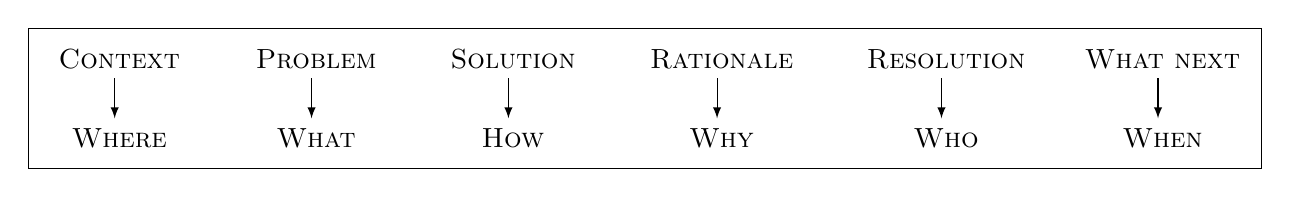
\begin{tikzpicture}[framed, dot/.style={circle,inner sep=1pt,fill,name=#1}]
\node (context) at (0, 0) {{ {\sc Context}}};
\node (problem) at (2.5, 0) {{ {\sc Problem}}};
\node (solution) at (5, 0) {{ {\sc Solution}}};
\node (rationale) at (7.65, 0) {{ {\sc Rationale}}};
\node (resolution) at (10.5, 0) {{ {\sc Resolution}}};
\node (whatnext) at (13.25, 0) {{ {\sc What next}}};

\node[below of=context] (where) {{ {\sc Where}}};
\node[below of=problem] (what)  {{ {\sc What}}};
\node[below of=solution] (how)  {{ {\sc How}}};
\node[below of=rationale] (why) {{ {\sc Why}}};
\node[below of=resolution] (who) {{ {\sc Who}}};
\node[below of=whatnext] (when)  {{ {\sc When}}};

\draw[-latex] (context) -- (where);
\draw[-latex] (problem) -- (what);
\draw[-latex] (solution) -- (how);
\draw[-latex] (rationale) -- (why);
\draw[-latex] (resolution) -- (who);
\draw[-latex] (whatnext) -- (when);
\end{tikzpicture}

\end{center}

%% The authors are part of a shifting, globally distributed, team of volunteers with around 30 major contributors, and a long tail with over 1000 members.\footnote{\url{https://plus.google.com/communities/107386162349686249470}} 
We believe that our pattern catalog will be useful for students and educators who want their work to have real-world relevance, to activists and policy-makers who want to develop practicable solutions to large-scale problems, and to employees and managers who, like it or not, find themselves working in distributed teams.   Our approach to emergent organization will also be of interest to theorists of social interaction in fields like organization studies and, increasingly, computer science.  The next section introduces the \patternname{Peeragogy Project} in the form of a design pattern.  Sections \ref{sec:Roadmap}--\ref{sec:Scrapbook} list the main patterns in our catalog.    Figure \ref{fig:connections} illustrates their interconnections.  Section \ref{sec:Distributed_Roadmap} summarizes the outlook.

\begin{figure}
\vspace{-.9in}
{\centering
\begin{tikzpicture}[dot/.style={circle,inner sep=1pt,fill,name=#1}]
%\draw[step=1cm,gray,very thin] (0,0) grid (10,10);
\node (assess) at (5, 9.75) {{\Large {\sc Assess}}};
\node (organize) at (5, 0) {{\Large {\sc Organize}}};
\node (cooperate)[text width=2cm,align=center,rotate=270] at (10, 5) {{\Large {\sc Convene}}};
\node (convene)[text width=15cm,align=center,rotate=90] at (0, 5) {{\Large {\sc Cooperate}}};
%%
\node (roadmap) at (4.25,4.65) {\ref{sec:Roadmap}. \emph{Roadmap}};
%%
\node (useormake) at (3.15, 8.75) {\ref{sec:Use_or_make}. \hyperref[sec:Use_or_make]{\emph{Use or make?}}};
\node (par) at (6.85, 8.75) {\ref{sec:Pattern_Audit_Routine}. \hyperref[sec:Pattern_Audit_Routine]{\emph{Pattern Audit Routine}}};
%
\node (carryingcapacity) at (1.25, 7.15) {\ref{sec:Carrying_capacity}. \hyperref[sec:Carrying_capacity]{\emph{Carrying capacity}}};
\node (heartbeat) at (1.6, 4.5) {\ref{sec:Heartbeat}. \hyperref[sec:Heartbeat]{\emph{Heartbeat}}};
%
\node (aspecificproject) at (8.5, 6.5) {\ref{sec:A_specific_project}. \hyperref[sec:A_specific_project]{\emph{A specific project}}};
\node (creatingaguide) at (6.85, 2) {\ref{sec:Creating_a_guide}. \hyperref[sec:Creating_a_guide]{\emph{Creating a guide}}};
%
\node (wrapper) at (2.5, 2) {\ref{sec:Wrapper}. \hyperref[sec:Wrapper]{\emph{Wrapper}}};
\node (newcomer) at (8.5, 3.25) {\ref{sec:Newcomer}. \hyperref[sec:Newcomer]{\emph{Newcomer}}};
\node (scrapbook) at (5, 1) {\ref{sec:Scrapbook}. \hyperref[sec:Scrapbook]{\emph{Scrapbook}}};
%
\node[below=2cm of newcomer] (peeragogyproject) {\ref{sec:Peeragogy_Project}. \emph{Peeragogy Project}};
%
\draw[-{Latex[width=2mm]},draw=gray] (peeragogyproject) -- ([xshift=0pt]newcomer.south);
\draw[-{Latex[width=2mm]},draw=gray] (aspecificproject) -- (par);
\draw[-{Latex[width=2mm]},draw=gray] (aspecificproject) -- (roadmap);
\draw[-{Latex[width=2mm]},draw=gray] (carryingcapacity) -- (newcomer);
\draw[-{Latex[width=2mm]},draw=gray] (carryingcapacity) -- (roadmap);
\draw[-{Latex[width=2mm]},draw=gray] ([xshift=2mm]creatingaguide.160) to[out=-215,in=-67] (carryingcapacity);
\draw[-{Latex[width=2mm]},draw=gray] (heartbeat) -- (newcomer);
\draw[-{Latex[width=2mm]},draw=gray] (heartbeat) -- (scrapbook);
\draw[-{Latex[width=2mm]},draw=gray] (heartbeat) -- (useormake);
\draw[-{Latex[width=2mm]},draw=gray] (newcomer) -- ([xshift=4mm]useormake.south);
\draw[-{Latex[width=2mm]},draw=gray] (newcomer) -- (aspecificproject);
\draw[-{Latex[width=2mm]},draw=gray] (newcomer) -- (creatingaguide.north);
\draw[-{Latex[width=2mm]},draw=gray] (newcomer) -- (roadmap);
\draw[-{Latex[width=2mm]},draw=gray] (par) -- (scrapbook);
\draw[-{Latex[width=2mm]},draw=gray] (roadmap) -- (newcomer);
\draw[-{Latex[width=2mm]},draw=gray] (roadmap) -- (useormake);
\draw[-{Latex[width=2mm]},draw=gray] (scrapbook) -- (par);
\draw[-{Latex[width=2mm]},draw=gray] (scrapbook) -- (wrapper);
\draw[-{Latex[width=2mm]},draw=gray] ([xshift=2mm,yshift=-.4mm]useormake.south) -- (creatingaguide);
\draw[-{Latex[width=2mm]},draw=gray] (wrapper) -- (heartbeat);
\draw[-{Latex[width=2mm]},draw=gray] (wrapper) -- (roadmap);
\end{tikzpicture}


\par
}
\vspace{-.9in}
\caption{Connections between the patterns of peeragogy.  An arrow points from pattern \textbf{A} to pattern \textbf{B} if the description of pattern \textbf{A} references pattern \textbf{B}. Labels at the borders of the figure correspond to the main sections of the \emph{Peeragogy Handbook}.\label{fig:connections}}
\end{figure}


\section{Peeragogy Project}

\begin{quote}
This section introduces the \emph{Peeragogy Project} in the form of a \emph{design pattern}.
\end{quote}

\paragraph{Context:}  Architectual maverick Christopher Alexander asked the following questions to an audience of computer programmers in 1999: 
\begin{quote}
``What is the Chartres of programming? What task is at a high enough level to inspire people writing programs, to reach for the stars?''
\end{quote}
We believe that the nexus of learning and computers -- exemplified today by Wikipedia, StackExchange, and Free/Libre/Open Source Software (FLOSS) -- presents an implicit challenge to the old way of doing things in education.  Taking up that challenge and building a new model is reaching \emph{ad astra per aspera}.  

\paragraph{Problem:} In a volunteer context, telling people what to do really doesn't work.  So we need another way to communicate.  Furthermore, everyone involved in these projects seems to be learning all the time.  So the way we communicate needs to be adaptive to circumstances.

\paragraph{Solution:} Christopher Alexander introduced the idea of \emph{design patterns} -- using a simple template to describe and shape the human life world.  In our context, design patterns allow us to bridge physical and virtual, move from fantastic to concrete and back.  The template we use is relatively traditional.  We've made a few minor alterations to Alexander's original model, in order to use patterns in a project that is always changing.  Specifically, we think of each pattern as something active: in addition to the traditional \emph{context}/\emph{problem}/\emph{solution} and \emph{rationale}, we try to make it clear what the very act of documenting each pattern \emph{resolves}, and we record the ``\emph{What's next}'' steps we have planned, in order to make the currently acting forces explicit. As time goes by we revise.  Like Alexander, we cross-reference our patterns to understand the links between them. The \emph{Peeragogy Project} is itself an up-to-date example of one of Alexander's patterns, \href{http://en.wikipedia.org/wiki/Networked_learning#1970s}{\emph{Network of Learning}} [APL].

\paragraph{Rationale:}
Patterns are intuitive to write and read. Our specific interpretation of the framework helps everyone involved integrate what they are learning.  We can use our design pattern catalog to scaffold our work on other parts of the project -- our technical platform, our Handbook, our meetings -- and to connect in fruitful ways with other projects.  

\paragraph{Resolution:}  
Writing down this pattern defines some of the key terms for \emph{Newcomers}, and illustrates the way our template works. 

\paragraph{What's next:} 
Feel free to join us and suggest new patterns and projects, or adapt our patterns to help shape another \emph{Peeragogy Project}.\footnote{In the present document, the term Peeragogy Project, without italics, refers to a current historical, real-world, example of the \emph{Peeragogy Project} pattern. This project has been active since it was introduced by Howard Rheingold in 2011. In order to enhance the readability of our patterns for a general audience, \emph{examples} drawn from our experiences in the Peeragogy Project and related projects, which would typically be part of a design pattern template, appear in footnotes.}
\begingroup \color{OliveGreen}

\section{Roadmap} \label{sec:Roadmap}

% DK: This is a bit self-referential. You have roadmap embedded throughout the description of the pattern. E.g. the context and problem should be able to describe the situation before the solution has been applied, so you should be able to describe them without the solution name in them.

% DK: How is this different from a Backlog? Who “owns” the roadmap? How are changes made to it? How precise is it? Does it have a time dimension to it? You refer to deadlines later on. Does the roadmap include them? (What do deadlines really mean in a project like this anyhow?) Priority?

\subsubsection*{Context} As discussed above, \patternname{Peeragogy} has both distributed and centralized aspects. In simplest terms, the several different discussants or contributors have different points of view and differing priorities, but they come together to share these in conversations and joint activities.

\subsubsection*{Problem} In order to collaborate, people need a way to share current, though incomplete, understanding of the space they are working in, and the nature of our relationships with one another and the other elemetns of this space.  Without a sense of personal goals, outstanding problems, and working methods, there is no way for people to volunteer to help out, or even to assess the project's progress.  

\subsubsection*{Solution} Keeping a list of current and upcoming activities, as well as goals and working methods can help \patternname{\href{http://peeragogy.org/practice/heuristics/newcomer/}{Newcomers}} and old-timers alike see where they can jump in.  This can take many forms, and can have different levels of detail.  The solution may take the form of an outline of a draft document, a backlog of issues in an issue tracker, a succinct organizational mission statement, a course syllabus, a manifesto, or a calendar of upcoming events.  The distinguishing feature of a roadmap in the peeragogical sense is that it must be adaptive to circumstances.  The roadmap should be accessible to everyone with an interest in the project, though in practice not everyone will choose to update it.  One of the jobs of the project's \patternname{Wrapper} is to help synthesize an accurate roadmap in lieu of widespread participation, or in case of conflict.

\subsubsection*{Rationale} Unless the project's plan is easy for people to see and to update, they are not likely to use it, and are less likely to get involved.  The roadmap can also impose other limitations, for example it may be ``owned'' exclusively by a central committee -- however the key point of the roadmap is to help support involvement by those who \emph{are} involved.  The opportunity for feedback (if this feedback is taken seriously) enhances a project's peeragogical aspects.  The level of detail in the roadmap (and the existence of a roadmap at all) should correspond to the felt need for sharing information and to the tolerance of uncertainty among participants.
% DK: This seems more like advice about how to implement the solution than it is an explanation of how the solution addresses the forces from the context/problem [jc: fixed]

\subsubsection*{Resolution}
% DK: This seems like Rationale to me [jc: fixed]
The roadmap can shift along with its contents: in the Peeragogy project it has ranged from an outline of the first draft of the Peeragogy Handbook to a calendar of meetings with a regular ``\patternname{Heartbeat}'' that has helped to sustain the project. Simply describing a list of nice-to-have features is not likely to \emph{go} anywhere: this shows the difference between a mere backlog of tasks and a realistic plan for getting from here, to there.  Only now with our latest strategy for using the pattern language as an organizational tool do we have a robust mechanism in place for building and maintaining a ``distributed roadmap.''

\begin{framed}
\emph{What's Next.}
If we sense that something needs to change about the project, that is a clue that we might need to record a new pattern.
\end{framed}

\endgroup
    
    
    
\begingroup \color{OliveGreen}

\begin{figure}
\begin{center}
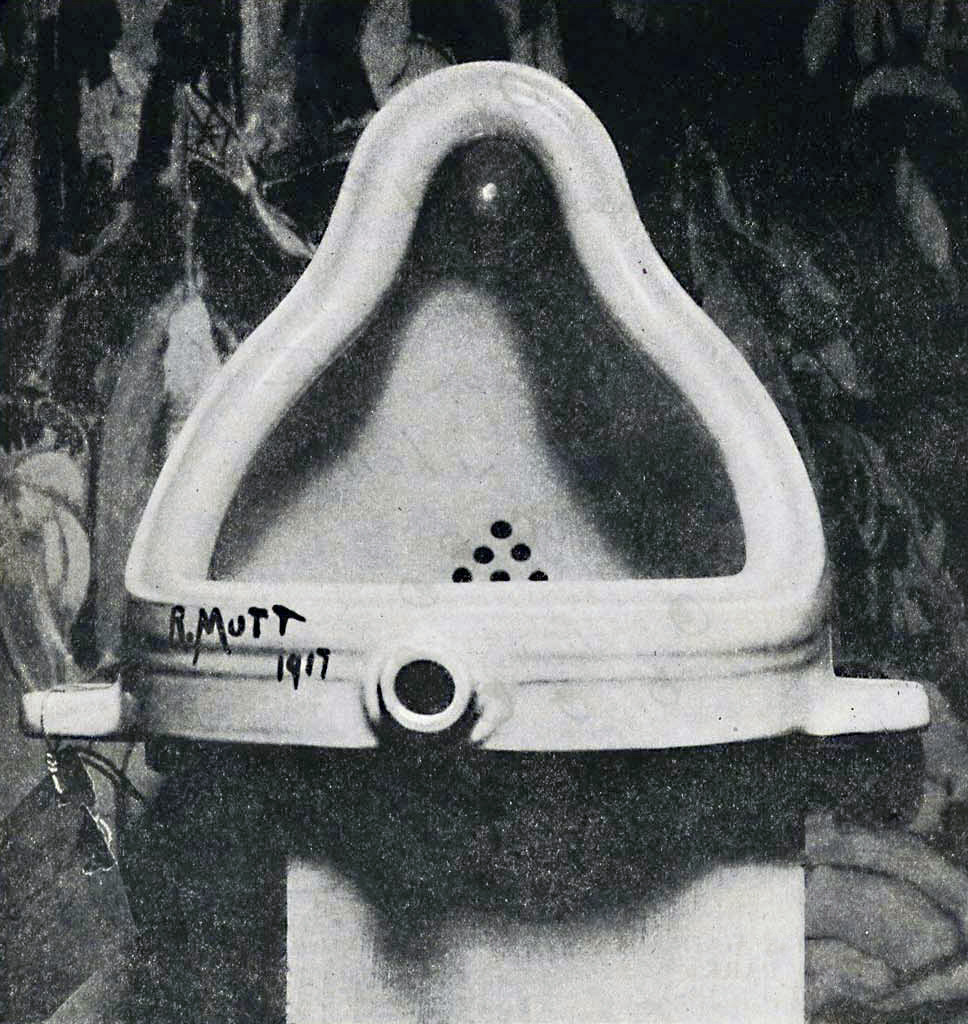
\includegraphics[width=.4\textwidth]{figures/Duchamp_Fountaine/Duchamp_Fountaine.jpg}
\end{center}
\caption{A paradigmatic example of found-art. Photograph by Alfred Stieglitz. Caption reads: ``Fountain by R. Mutt, Photograph by Alfred Stieglitz, THE EXHIBIT REFUSED BY THE INDEPENDENTS''. Public domain, via the Wikimedia Commons.\label{fountain}}
\end{figure}

\section{Don't make what you can simply use, and don't sell what you can afford to give away} \label{sec:Use_or_make}
% DK: I am not sure about the [old] title of this pattern. The bulk of the body of the pattern seems to be about the reuse. Maybe something like “Don’t Make what you can Use” might fit the spirit better. [fixed]

\subsubsection*{Context}
% DK: This seems like an explanation of the title, not a context in which a problem is observed.
Peer production, as the name indicates, is about producing, in other words -- ``making stuff.''  Similarly, in academia, it's all about making an ``impact,'' and in business usually has something to do with making money.  But we only ever do any of this by building on the work of others.    

\subsubsection*{Problem}
People are often very attached to their own projects and priorities and don't have a sense of how their initiatives can benefit from connecting with others. Many projects die because the cost of \patternname{\href{http://c2.com/cgi/wiki?ReinventingTheWheel}{Reinventing the Wheel}} [c2] is too high.  We're often blind to the obstacles that we put in our own path.

\subsubsection*{Solution} Learning something new generally involves connecting deeply with what's already there.  While it's a great idea to ``steal like an artist'' don't forget to return the favor and make it possible for other people to remix and adapt your work too (Figure \ref{fountain}).  One good start is to give it away, then it's not technically stealing when others use it.
%\cite{anderson2009free}.
In our case, we've released the \emph{Peeragogy Handbook} using the Creative Commons Public Domain Dedication (CC0), a legal instrument grants the greatest possible leeway to downstream users.\footnote{\url{https://creativecommons.org/publicdomain/zero/1.0/}}  Show appreciation when someone takes up the offer.  (In the case of shared content, make backups so that you don't have to worry about losing the record of idea that another person might not have noticed was important.)

\subsubsection*{Rationale} 
Clearly we are not the first people to notice the problems with wheel-reinvention, including ``missing opportunities, repeating common mistakes, and working harder than we need to.''\footnote{\url{https://blog.wikimedia.org/2013/11/19/learning-patterns-new-way-share-important-lessons/}}  As Willow Brugh of Geeks without Bounds and the MIT Media Lab remarked as a guest in one of our hangouts\footnote{\url{https://www.youtube.com/watch?v=NpyQfYVKfBI}}: people often think that they need to build a community, and so fail to recognize that they are already part of a community.  Just as there can be subsequent benefits to helping your neighbor, it behooves us well to serve the communities that we are part of, rather than ignore them.   When we re-purpose the work of others, we potentially create a new bond.   When we think about how others can leapfrog ahead by building on our experiences, we prepare for something similar in the future.

\subsubsection*{Resolution}   It's worth keeping in mind that peeragogy per se is not new, and it's not something we can bottle and sell.  But we can try to learn how to do it more effectively.  Innovation doesn't come out of the blue -- and furthermore, as much as innovation is celebrated in our culture, there's something to be said for tradition, too.   The pattern \patternname{Don’t make what you can simply use, and don’t sell what you can afford to give away} can help guide us toward shared language and mutual understanding.  This is the often best way to help get around those nasty self-defeating obstacles.

\begin{framed}
\emph{What's Next.}
We've spun off the pattern catalog from the \emph{Peeragogy Handbook} into this paper, sharing it with a new community and gaining new perspectives.  Let's look for other parts of the handbook we can spin off!
\end{framed}

\endgroup

\section{Carrying capacity}\label{sec:Carrying_capacity}
\subsubsection*{Definition} There's only so much any one person can do in a
project.

\subsubsection*{Problem} At times, a facilitator or participant in the
peer-learning enterprise may feel he or she is over-contributing -- or,
perhaps more likely, that others are under-contributing -- or that
someone else is railroading an idea or dominating the discussion.

\subsubsection*{Solution} If this happens, take a step back and observe the
dynamics of involvement. Ask questions and let others answer. Especially
if you start to feel the symptoms of burnout, it's important that you
find the level of engagement that allows you to participate at a level
that is feasible for maintaining progress toward the project's goal.
Lead by example -- but make sure it's someplace you, and others,
actually want to go! This could be a good time to revisit the group's
roadmap and see if you can figure out and clarify to others what
concrete goal you're working towards. Remember that you can also change
the ``landscape'' by making it easier for other people to get involved
-- for example, by explaining what you're trying to do in a clear
manner. Be on the look out for opportunities to step back, watch, and
listen. Try to be mindful of phases when active or quiet involvement
would be more helpful to the individual and the group. It's also helpful
to let anyone who has taken on a facilitation role know if you're
stepping back temporarily. Then, when the time is right, step back in
and get to work!

\subsubsection*{Challenges} Even though your project may be very important, you
won't always make it go better by working harder.

\begin{quote}
\textbf{Alvin Toffler}: If overstimulation at the sensory level
increases the distortion with which we perceive reality, cognitive
overstimulation interferes with our ability to `think.'
\end{quote}

If you notice yourself caring about the outcomes more than other
participants, investigate why this is. Are you all affected by the
outcomes in the same way? Working smart requires you to focus on your
goals, while relating to others who may have a different outlook, with
different, but still compatible goals.

\subsubsection*{What's Next} This pattern catalog has been rewritten in a way
that should make it easy for anyone to add new patterns. Making it easy
and fruitful for others to get involved is one of the best ways to
redistribute the load (compare
the \patternname{\href{http://peeragogy.org/practice/heuristics/newcomer/}{Newcomer}}
pattern).



\section{A specific project}\label{sec:A_specific_project}
\subsubsection*{Context}
You find yourself interested in or concerned about something, but you
only have a vague idea about how it works or how you fit in.

\subsubsection*{Problem}
It's easy to think about issues that matter: there are many of
them. The problem is figuring out what you're going to do about it.
As a further problem, getting concrete can be scary, because you risk
failure.\footnote{In the Peeragogy project and more broadly, we've
  observed that some people are happy with a sense of experience or
  process, while others want to see results. Some others are in the
  middle.  All of these variations are OK!  However, we are often
  blinded by our own preferences, and in the worst case this can
  undermine or destroy group dynamics.  At the very least it will add
  tension, as some want to continue to discuss and engage generally
  while others want to move forward.  When the forward-movers try to
  act, those enjoying the experience may attempt to shut them down or
  may feel that they are being left out/behind.}

\subsubsection*{Solution} 
If you \emph{are} able to get concrete about something to do, learn, and achieve, you move from thinking about a topic to becoming a practitioner.  You may realize that your ``specific project'' is too large to tackle directly. In this case, you will have to become even more specific.  Maintaining a project \patternname{Roadmap} can help keep track of the smaller pieces and the bigger picture.

\subsubsection*{Rationale} 
Being specific is important for bringing about to change.\footnote{In the January, 2013, plenary
session, \href{http://ipne.org}{Independent Publishers of New England}
(IPNE) President Tordis Isselhardt quietly listened to a presentation
about how we created the \emph{Peeragogy Handbook}. During the Q\&A, she
spoke up, wondering if peer-learning effort in IPNE might be more likely
to succeed if the organization's members ``focused around a specific
project.'' As this lightbulb illuminated the room, those of us attending
the plenary session suggested that IPNE could focus the project by
creating an ``Independent Publishing Handbook.'' (Applause!) In the
course of creating the IPNE Handbook, peer learners would assemble
resource repositories, exchange expertise, and collaboratively edit
documents. To provide motivation and incentive to participate in
``PeerPubU'', members of the association will earn authorship credit for
contributing articles, editor credit for working on the manuscript, and
can spin off their own chapters as stand-alone, profit-making
publications.} But while actions speak louder than words, it's important
to act in a coherent way if you want to be understood by others.  However, in
general it would be a mistake to try to seek consensus before acting: it's much better to combine action with dialog.

\subsubsection*{What's Next}  Each project connected with the Peeragogy Project should be described with one or more patterns, each with specific, tangible ``what's next'' steps.\footnote{We've found that writing papers for conferences is one activity that can help us focus and make improvements to our body of work that would not come about by simply meandering through revisions to the \emph{Peeragogy Handbook}.  Remixing these efforts into the handbook is a good source of improvements; see \patternname{Use or Make}.}  The \patternname{Pattern Audit Routine} can help make these ``what's next'' steps concrete. 


\section{Wrapper}
\paragraph{The Definition:} The wrapper role can be taken on by a project
participant who summarizes everything going on in the project, making
the project comprehensible to participants who haven't been following
all of the details.

\paragraph{The Problem:} Joining the project that is already going can feel
like trying to get aboard a rapidly moving vehicle. If you've joined and
then taken time off, you may feel like things have moved on so far that
it's impossible to catch up. In a very active project, it can be
effectively impossible to stay up to date with all of the details.

\paragraph{The Solution:} Charlie
Danoff \href{http://socialmediaclassroom.com/host/peeragogy/wiki/rolesdivision-labor}{suggested}
that someone take on the ``wrapper role'' -- do a weekly pre/post wrap,
so that new (and existing) users would know the status the project is at
any given point in time. The
project's \href{http://socialmediaclassroom.com/host/peeragogy/}{landing
page} also serves as another sort of ``wrapper'', telling people what
they can expect to find.

\paragraph{Objectives:} In fulfilling the wrapper role, we must check the
public summaries of the project from time to time to make sure that they
accurately represent the facts on the ground.\footnote{In the first year of the Peeragogy project, the
``Weekly Roundup'' by Christopher Tillman Neal served to engage and
re-engage members. Peeragogues began to eager watched for the weekly
reports to see if our teams or our names had been mentioned. When there
was a holiday or break, Chris would announce the hiatus, to keep the
flow going. In the second year of the project, we didn't routinely
publish summaries of progress, and instead, we've assumed that
interested parties will stay tuned on Google+. Nevertheless, we maintain
internal and external summaries, ranging from agendas to press releases
to quick-start guides. Regular meetings provide an alternative way to
stay up to date: see
the \href{http://peeragogy.org/patterns/heartbeat/}{Heartbeat} pattern.}

\paragraph{Challenges:} According to the theory proposed by Yochai Benkler,
for free/open ``commons-based'' projects to work, it is vital to have
both (1) the ability to contribute small pieces; (2) something that
stitches those pieces together {[}1{]}. The wrapper performs this
integrative function, which is often much more challenging than the job
of breaking things down into pieces or just doing one of the small
pieces.

\paragraph{What's Next:}
We need better practices for wrapping things up at
various levels.  One of the latest ideas is to develop a simple visual
``dashboard'' for the project.

\paragraph{Reference:}

\begin{enumerate}
\itemsep1pt\parskip0pt\parsep0pt
\item
  Benkler, Y.
  (2002). \href{http://www.yale.edu/yalelj/112/BenklerWEB.pdf}{Coase's
  Penguin, or Linux and the Nature of the Firm}, Yale Law Journal 112,
  pp. 369-446.
\end{enumerate}

\section{Heartbeat}

\paragraph{Context:}
People have a shared interest, and have connected with each other about it.

\paragraph{Problem:} What's an easy way for these people feel like there's a ``there, there?''

\paragraph{Solution:} People seem to naturally gravitate to regularly scheduled
activities. Once a week (meetings) or once a year (conferences) are two common variants.  Sometimes people need a little extra prompt to join in.\footnote{In the ``Collaborative Lesson Planning'' course led
by Charlie Danoff at P2PU, Charlie wrote individual emails to people who
were signed up for the course and who had disappeared, or lurked but
didn't participate. This kept a healthy number of the people in the
group to re-engage and make positive contributions. In more recent
months, Charlotte Pierce has been running weekly meetings by Google
Hangout to coordinate work on the \emph{Peeragogy Handbook} and tend to other community interests. Not only have we
gotten a lot of hands-on editorial work done this way, we've generated a
tremendous amount of new material (both text and video footage) that is
likely to find its way into future versions of the \emph{Peeragogy Handbook}.  As long as this continues, ``Mondays at 1PM Eastern US time'' is a reliable time to make contact with the Peeragogy Project.}

\paragraph{Rationale:}  This pattern might seem too obvious, since regularly scheduled meetings are so ubiquitous.  But there's an important difference between a mere meeting and a \emph{Heartbeat}: in short, if the energy from your meetings isn't helping you or your group thrive, something needs to change.

\paragraph{Resolution:} This pattern is one of the easiest to explain to \emph{Newcomers} to the idea of design patterns, since nearly everyone is familiar with the pattern of regular routine.  But the pattern is also a sophisticated tool: noticing when a new \emph{Heartbeat} occurs is a way to be aware of the priorities in the group, and may be a good source of new patterns.

\paragraph{What's Next:} When the project is bigger than more than just a few people, it's likely to have several \emph{Heartbeats}\footnote{There have been several periods of time operated two regularly scheduled weekly meetings in the Peeragogy project at distinct times, for members with slightly different interests and slightly different availability.  This typically relates to small special-purpose projects, like our work on this paper.}  Identifying and fostering new \emph{Heartbeats} and new working groups is a task that can help make the community more robust.

\section{Creating a guide}\label{sec:Creating_a_guide}
\subsubsection*{Context} Meaning-carrying tools, like handbooks or maps, can help collect content and stories as well as assist others who want to adopt the idea, .

\subsubsection*{Problem} 
Established ideas have knowledge cartography challenges for newcomers, consider trying to decipher a subway map in a foreign city. When the idea or system is only ``newly discovered'', the associated meanings may not be well understood, and indeed they may not have been created. Even if a topic is only ``personally new'', it can be hard to find one's way around.

\subsubsection*{Solution}
The process of creating the guide can go hand-in-hand with figuring out how the system works. Thus, techniques of \href{http://knowledgecartography.org/}{knowledge cartography} and \href{http://www.hitl.washington.edu/publications/r-97-47/two.html}{meaning making} are useful for would-be guide creators.\footnote{We started the Peeragogy project by collaboratively making an outline for the Peeragogy Handbook. We recommended this
handbook-making practice to others, as a way to learn collaboratively and build a strong group.}

\subsubsection*{Rationale} 
It is important to keep in mind how ``the map is not the territory,'' and map-making is only one facet of shared human activity. For instance, a pattern description can be thought of as a ``micro-map'' of a specific activity. These maps are not useful if they are divorced from practice.

\subsection*{Resolution}
As \href{https://www.gnu.org/philosophy/free-doc.html}{Richard Stallman} wrote about free software documentation, 

\begin{quote}
"The biggest deficiency in free operating systems is not in the software—it is the lack of good free manuals that we can include in these systems. The biggest deficiency in free operating systems is not in the software—it is the lack of good free manuals that we can include in these systems. Many of our most important programs do not come with full manuals. Documentation is an essential part of any software package; when an important free software package does not come with a free manual, that is a major gap." it is of vital importance to create a guide for your idea if you want others to adopt it for use.
\end{quote}

Without a guide it is far less likely for an idea to become adopted by others. The process of creating a guide creates a certain formality to the project, forcing participants to catalogue and explicate their idea. Additionally, the act generally leads to deadlines which can help prod individuals to work on the project ore regularly.

\subsubsection*{What's Next} 
Working with our shepherd at PLoP to improve this paper!



\section{Newcomer}
\subsubsection*{Context:}
A lot of ``education'' assumes we are speaking to a new generation. 
In learning more broadly, the ``audience'' is often new to the topic.
Sometimes we are the \emph{Newcomers}, sometimes we're the oldtimers.

\subsubsection*{Problem:} \emph{Newcomers} can feel overwhelmed by the amount of things to learn.  They
don't know where to start.\footnote{Peeragogy Project participant
R\'egis Barondeau: ``I joined this handbook project late, making me
a `newcomer'. When I started to catch up, I rapidly faced doubts:
Where do I start? How can I help? How will I make it, having to read
more than 700 posts to catch up? What tools are we using ? How do I use
them? Etc. Although this project is amazingly interesting, catching the
train while it already reached high speed can be an extreme sport. By
taking care of newcomers, we might avoid losing valuable contributors
because they don't know how and where to start, and keep our own project
on track.''}  They may have a bunch of ideas that the oldtimers have
never considered -- or they may think they have new ideas, which are actually
a different take on old ideas; see \emph{Use or Make}.

\subsubsection*{Solution:} It is good to try to become aware of what a \emph{Newcomer}
needs, and what their motivations are.\footnote{Peeragogy Project participant
Charlotte Pierce: ``Joe was working a lot on the book, and I thought
`this is interesting hard work, and he shouldn't have to do
this alone.' As a Peeragogy newcomer, I was kindly welcomed and
mentored by Joe, Howard, Fabrizio, and others. I asked naive questions
and was met with patient answers, guiding questions, and resource links.
Concurrently, I bootstrapped myself into a position to contribute to the
workflow by editing the live manuscript for consistency, style, and continuity.''}
\emph{Newcomers} themselves may have only a general idea about what their goals are, so it can be
helpful to add concreteness with \emph{A Specific Project}.

\subsubsection*{Rationale:} \emph{Newcomers} in the Peeragogy project have often complained
about feeling confused about what the project is about, suggesting that our \emph{Roadmap}
has not been sufficiently clear.  Some feel it is too theoretical, which suggests
we need to do more work on \emph{Creating a guide} on ways to get involved, while also
making it clear that we do not have an exhaustive list in mind.  New ideas can prompt us to consider how we may have been limiting ourselves.\footnote{Dilrukshi Gamage, Julia Echeverria, and Federico Monaco first joined a Peeragogy hangout in February, 2015.  They were all interested in the idea of designing and running a course on peer learning.  Although we had done some work on a syllabus, and considered the notion of using peeragogical models in formal education, we hadn't tried running a course on the topic of peeragogy.  There were a number of earlier experiments that \emph{used} ideas from peeragogy inside of a formal course, and the difference between these two approaches prompted interesting discussions.}

\subsubsection*{Resolution:}
The frustration and confusion felt by a \emph{Newcomer} familiar to anyone who is starting something new.  An awareness of how to help \emph{Newcomers} can help us be more compassionate to ourselves and others.

\subsubsection*{What's Next:} A more detailed (but non-limiting) ``How to Get Involved'' walk-through in text or video form would be good to develop. We can start by listing some of the things we're learning about.\footnote{Business issues relevant to the Peeragogy project, how to run a MOOC, etc.}

\section{Pattern Audit}

\subsubsection*{Context:} Our collection of patterns grows.

\subsubsection*{Problem:} This becomes confusing.  Not all of the patterns are equally relevant.

\subsubsection*{Solution:} Periodically run a pattern audit.  Bring in a real-time aspect using the Paragogical Action Review.  Any patterns that can't be made relevant for our current interests can be moved to the \emph{Scrapbook}

\subsubsection*{Rationale:} We want to keep the attention focused on the most relevant issues.

\subsubsection*{Resolution:} Writing this down helps us describe our effort to focus.

\subsubsection*{What's Next:} Get some practice with the \emph{Audit} pattern in our next meeting.

\section{Scrapbook}

\paragraph{Context:} We've maintained and revised our pattern catalog over a period of years.
\paragraph{Problem:} Some of the patterns don't seem to lead to concrete next steps.
\paragraph{Solution:} We've created a \emph{Scrapbook} for patterns that are no longer part of the active catalog.  It's worth remembering how we got to the point we're at now, and the thinking that developed along the way, so the \emph{Scrapbook} shows some patterns that seemed like a good idea at the time -- and brief notes about why we no longer need them explicitly.  We can use the \emph{Pattern Audit Routine} to decide when to move a pattern into the \emph{Scrapbook}.
\paragraph{Rationale:} We want our collection of patterns to be concretely useful and actively used.  It needs to be clear and pragmatic, and not overly theoretical or precriptive.  If we don't see ``what's next'' and where it came from, then it's probably time to shift focus to something else more practical.
\paragraph{Resolution:}  In revising our pattern catalog for PLoP we've decided to ``retire'' several patterns that seemed overly abstract or redundant (\emph{Discerning a pattern}, \emph{Polling for ideas}, \emph{Moderation}, \emph{Roles}) as well as some antipatterns that didn't suggest concrete next steps, and instead simply held a prism to our collective frustrations (\emph{Isolation}, \emph{Magical thinking}, \emph{Messy with Lurkers}, \emph{Misunderstanding power}, \emph{Navel Gazing}, \emph{Stasis}, \emph{Stuck at the level of weak ties).  The current catalog is leaner and redescribes our project in an action-oriented way. 
\paragraph{What's next:} After significantly pruning back the pattern catalog, we want it to grow again: new patterns are needed.  Reviewing the contents of the \emph{Scrapbook} will be one place to look for inspiration, but there are others.


\section{Distributed Roadmap} \label{sec:Distributed_Roadmap}

\begin{quote}
This section summarizes the ``What's Next'' steps in all the previous
patterns, reprising the \emph{Roadmap} in a distributed, emergent form.
\end{quote}

\subsubsection*{Roadmap} Adding ``What's Next'' steps to our patterns gives us a ``distributed roadmap'' for the \emph{Peeragogy Project}.  And this works both ways:  
If we sense that something needs to change about the project, that's a
clue that we might need to record a new pattern.

\subsubsection*{Use or make} 
We've spun off the pattern catalog from the \emph{Peeragogy Handbook} into this paper, sharing it with a new community and gaining new perspectives.  Let's look for other parts of the handbook we can spin off!

\subsubsection*{Carrying capacity} This pattern catalog has been rewritten in a way that should make it
easy for anyone to add new patterns. Making it easy and fruitful for
others to get involved is one of the best ways to redistribute the load
(compare the Newcomer pattern).

\subsubsection*{A specific project} 
 Each project connected with the \emph{Peeragogy Project} should be described with one or more patterns, each with specific, tangible ``what's next'' steps.  The \emph{Pattern Audit Routine} can help make these ``what's next'' steps concrete.

\subsubsection*{Wrapper}  We need better practices for wrapping things up at
various levels.  One of the latest ideas is to develop a simple visual
``dashboard'' for the project.

\subsubsection*{Heartbeat} When the project is bigger than more than just a few people, it's likely to have several \emph{Heartbeats}.  Identifying and fostering new \emph{Heartbeats} and new working groups is a task that can help make the community more robust.  This is the temporal dimension of spin off projects described in \emph{Use or Make}.

\subsubsection*{Creating A Guide} We’ve been talking with collaborators in the Commons Abundance Network
about how to make a Pattern Language for the Commons. One of the
challenges that arises is how to support ongoing development of the
Pattern Language itself: a “living” map for a living territory. We’re
refining the Peeragogy Pattern language and template as a seed for this.

\subsubsection*{Newcomer} A more detailed (but non-limiting) ``How to Get Involved'' walk-through in text or video form would be good to develop. We can start by listing some of the things we're learning about.

\subsubsection*{Pattern audit routine}  TBA

\subsubsection*{Scrapbook} After significantly pruning back the pattern catalog, we want it to grow again: new patterns are needed.  Reviewing the contents of the \emph{Scrapbook} will be one place to look for inspiration, but there are others.





\bibliographystyle{acmlarge}
\bibliography{peeragogy-bib}

% Appendix
\elecappendix
\section{``Peeragogy'' or ``Paragogy''?}

I want to attach a marginal note, as it were, to our article on
Patterns of Peeragogy.  First, an etymological fragment:

\begin{quotation}
The prefix \emph{para-} meaning beside is Greek, and the prefix \emph{para-}
meaning \emph{against} is French, stemming from the Latin word \emph{parare} (to
make ready) unrelated to the Greek \emph{para-}. No shift of meaning, just a
coincidence.\footnote{Peter Shor, at \url{http://english.stackexchange.com/questions/54673/why-is-para-not-used-consistently}}
\end{quotation}

Another (rather convenient) coincidence: ``paragogy'' is an existing
Greek word, meaning production.  I always liked the implied double
meaning that paragogy was about both ``peer learning'' and
``production.''  The gloss ``peer produced peer learning'' puts the
emphasis on peer \emph{learning}, and with ``peeragogy'' the
dual-language pun is gone entirely.  Still, it would be good if
the ``production'' aspects got fair play.  With these comments in
mind, consider:

\begin{quotation}
Opposition can be the law of the relation between abstract products,
but difference is the only principle of genesis or production; a
principle which itself produces opposition as a mere appearance.
Dialectic thrives on oppositions because it is unaware of far more
subtle and subterranean differential mechanisms. \citeadx[p. 157]{deleuze2006nietzsche}
\end{quotation}

Here we have ``para-'' in both its Greek and its Latin forms, opposed
but in a particularly subtle way.  Gilles Deleuze is saying that
``thesis/antithesis/synthesis'' isn't how consciousness comes into
being \citeadx[p. 34]{hughes2009deleuze}.  Rather, it is as if consciousness and
being itself feels its way forward, distinguishing the present from
the past, creating new forms and re-creating individual beings as it goes.  So
another very philosophical way to read the word ``paragogy'' would be
to think of this Deleuze quote and our participation in the genesis of
being!

\section{Patterns and dynamics}

We can assert that in getting into a tangle with things we are ``doing
philosophy'' in a Deleuzian manner.  With regard to the design pattern catalog, we are not just thinking of
\emph{abstract} patterns, but patterns that are contingent on what we
do, and patterns that -- as we distinguish them -- shape who we are.
The way we use design patterns  ``constitutes and occupies practical or
speculative problems as such'' \citeadx[p. 204]{deleuze1994difference}
-- and this centrally involves learning .  Something of this dynamical view
is developed by Christian Kohls in
\citeadx{kohls2010structure,kohls2011structure}, but in a less
``embedded'' sense.


\bibliographystyleadx{acmlarge}
\bibliographyadx{peeragogy-bib}


\end{document}
